\documentclass[10pt, a4paper]{article}
\usepackage{graphicx} 
\usepackage{multicol}
\usepackage{enumitem}
\usepackage{float}
\usepackage[left=25mm, top=20mm, right=25mm, bottom=20mm, nohead, footskip=15mm]{geometry}
\pagestyle{plain}
\setcounter{page}{249}
\usepackage{amsmath}


\begin{document}

\begin{multicols}{2}
the sensitive measure, in which more information is
included\
\begin{center}
    III. PROPOSED HAND GESTURE RECOGNITION
METHOD

\end{center}
 \ \ \ The general block scheme of hand gesture recognition
includes the following components, which are static hand
gesture dataset, binary and skeleton image formation,
feature labeling and extraction, classifier models, and
performance evaluation. This general blcok-scheme is
presented in Fig. 1, all major components are marked
with green color.

 \ \ \ Static hand gesture images are stored in the images
dataset. They are used to train the classifier and evaluate
the accuracy of the classification task. These RGB images of hand gestures are first passed into a block that
can form the binary and skeleton images from them. All
the proposed skeletonization and denoise methods are
embedded in this block.

 \ \ \ Next, feature extraction is conducted based on these
obtained binary and skeleton images. For each pair of
binary image and skeletal image, there are nine geometry
features should be extracted, and they together compose
a feature vector. Next, manual labeling for each pair of
binary and skeleton images is also required to get the
truth labels that corresponding to each feature vector.
These feature vector can passed to the trained classifier
for prediction. By comparing the predicted label and the
truth label to compute the accuracy. In the classification
module, there are six different well-known classifiers
for optional, which includes decision tree(DT) [31], knearest neighbors (KNN) [32], naïve Bayes (NB) [33],
support vector machine (SVM) [34], ensemble learning
(EL) [35], multilayer perceptron (MLP) [36].\\

A.\textit{Creation of the Hand Gesture Dataset}\\

 \ \ \ All static hand gesture images that in dataset are
captured with the iPhone 11. The resolution of images are
3024 × 3024 × 3. Since directly processing these images
is time-consuming, resize operation is used to converting
these images into 95×95×3 images. The dataset consists
of ten different classes, example pictures are shown in
Fig. 2.

 \ \ \ In each one class, there are more than 100 different
images. As a result, the total amount of our dataset is
over 1000 images. These images are randomly divided
into train-validation group and testing group. The number
of images in testing group is equal to 20\% of the initial
image set, and the number of images in train-validation
group is 80\% of the initial image set. \\

B. \textit{Forming Binary Image and Skeleton Image using Hybrid Combining Denoising Techniques and Skeletonization Methods}
\par
 \ \ \ The skeleton and pattern images are extracted from
the original images by using different combinations of



\begin{figure}[H]
    \centering
    \includegraphics[width=0.94\linewidth]{image1.png}
    \caption{ \small {Example of the Ten Class of Hand Gestures.}}
    \label{fig:enter-label}
\end{figure}

skeletonization method and denoise methods . There are
six hybrid methods are used, which including ZS+ATFM,
OPTA+ATFM, OPCA+ATFM, ZSM+ATFM,
MOPCA+ATFM, and MOPCA+ATFM+DCEM. The
time consumption of these methods is listed in Tab. I.
\par
From Tab. I, it is noted that ZS+ATFM,
OPTA+ATFM, ZSM+ATFM, MOPCA+ATFM, and
MOPCA+ATFM+DCEM respectively spend more 38\%,
22\%, 33\%, 0.4\%, and 5\% time when compared with the
method of OPTA+ATFM. Besides, we can learned the
use of DCEM may take extra 0.02 seconds.
\par
In Fig. 3, we listed example skeletons extracted from
\newpage
\begin{table}[H]
\caption{\label{tab:canonsummary}}TIME CONSUMPTION OF SIX METHODS
\begin{center}
\begin{tabular}{|c|c|}
\hline
\textbf{Skeleton Image} \\
\textbf{Extract algorithm}
& 
Average Time of 


\\




\hline
\textbf{ZS+ATFM} & 0.704 \\
OPTA+ATFM & 0.624 \\
OPCA+ATFM & 0.510\\

ZSM+ATFM & 0.682 \\
MOPCA+ATFM & 0.512 \\
MOPCA+ATFM+DCEM & 0.536\\
\hline
\end{tabular}
\end{center}
\end{table} 
he images that are shown in Fig 2 by using the skeletonization method MOPCA with both ATFM and DCEM.
\begin{figure}[H]
    \centering
    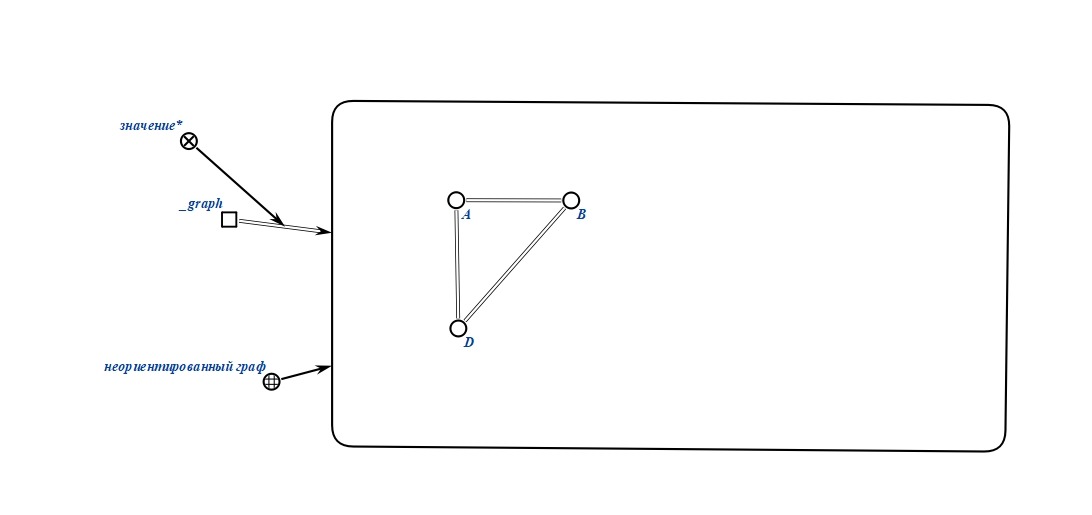
\includegraphics[width=0.87\linewidth]{image.png}
    \caption{ \small { Skeleton examples of ten hand gesture classes.}}
    \label{fig:enter-label}
\end{figure}
C. \textit{Feature extraction based on Skeleton and Binary
Images}\\
\par
 After a skeletal image and its pattern image are obtained from an input image, it is necessary to transform
the skeletal images along with its pattern image to a
9-dimension feature vector used in the later classification. This 9-dimension vector includes the following
significant geometrical features: the number of endpoints
(NEP); the number of cross points (NCP); the existence
of the inner hole (EIH); the average virtual-real distance
rate between each pair of endpoints (AVRD); the number
of virtual cross points (NVCP); Rate of the deviation
of the thick of the endpoints (RDTE); Average distance
between the thickest point in a pattern image and each
endpoint in the skeletal image(ADTPE); distance between pattern thickest point and skeletal thickest point
(DPSP); average angle of the endpoint (AAEP). Each
dimension of this feature vector is manually selected with
respect to the topology of these different classes.
\par
The NEP is obtained by summarizing the number of
these foreground pixels, which have only one neighbor
foreground pixel in its 8-neighborhood window in the
skeletal image.
\par
The NCP is obtained by summarizing the number
of these foreground pixels, which have more than two
neighbor foreground pixels in its 8-neighborhood window in the skeletal image.
\par The EIH is an important geometry feature with only
two values, 0 or 1. The inner hole denotes that the hole
should be enclosed by the skeleton. Ideally, only Class 7
and Class 10 have the inner hole. One method to judge
the existence of the inner hole for these hand images is
to compute the number of closed areas in the skeleton
image.
\par
The AVRD describes the similarity of the real connecting line between endpoints to the virtual closet straight
line between them. For each pair of endpoints, the real
connecting line and its distance can be obtained using
breadth-first search (BFS) algorithms, and the distance of
the virtual line is calculated using the Euclidean distance
formula. Then the average value is easily obtained.
\par The NVCP is obtained by summarizing the total
number of points at the intersection of the virtual line
and the real line.
\par
Before presenting the definition of RDTE, ADTPE,
and DPSP, the concept of thickness is first introduced.
The thickness of a pixel is defined by the distance
between this pixel and its closest pixel located on the
boundary in the pattern image. Boundary pixels comprise
the foreground pixel, whose four neighbors have at least
one background pixel.
\par
For a given skeleton with n endpoints, all endpoints
can form a set SEP , in which the i-th endpoint is denoted
as SEPi
. The thickness of SEPi
can be denoted as TEPi
.
The set formed by all TEPi
is denoted as TSEP . Then,

\end{multicols}

\newpage
\begin{figure}
    \centering
    \includegraphics[width=1\linewidth]{image3.png}
    \caption{Classification Models and Performance Evaluation.
}
    \label{fig:enter-label}
\end{figure}
\begin{multicols}{2}
the RDTE for this skeleton can be computed by using
the following formula
\par
RDTE = \begin{cases}0 & n \leq 1\\\sum_i^n \sqrt{\frac{(T_{EP_{i}}-\frac{1}{n}\sum_i^n T_{EP_{i}})^2}{\max({T_{S_{EP}}})-\min{(T_{S_{EP}}})}} & n > 1\end{cases}
\par
We suppose the coordinates of the thickest pixel in the
pattern image are Px and Py, and its thickness is Tp. We
suppose that in a skeletal image, there are n endpoints.
The coordinates of the i-th endpoint are denoted as EPix
and EPiy
. Then, the ADTPE can be calculated by using
the following formula:
\par
AMDTE = \begin{cases}0 & n \leq 1\\\sum_i^n \sqrt{\frac{(T_{EP_{i}}-\frac{1}{n}\sum_i^n T_{EP_{i}})^2}{\max({T_{S_{EP}}})-\min{(T_{S_{EP}}})}} & n > 1\end{cases}
\par
Supposing the coordinate of the thickest pixel in the
pattern image is Px and Py, and the coordinate of
the thickest pixel in the skeletal image is Sx and Sy,
the DPSP can be calculated according to the following
formula:\\
\par
DPSP = \sqrt{(P_{x}-S_{x})^2+(P_{y}-S_{y})^2}\\
\par
Before obtaining the value of the AAEP, the main
axis is defined by the thickest point in the pattern image
and the farthest endpoint in the skeletal image from that
point. Based on that, it is easy to calculate the relative
angle of the remaining endpoint to these axes, and the
AAEP is the mean of these angles. If the number of
endpoints is less than 2, the AAEP is set as 0.\\
\par
D. \textit{ Classifier Models and Performance Evaluation}\\
\par
The obtained feature vectors of the images from the
training set of the dataset and their labels are passed to
classifiers metioned, then conduct the learning process.
The hyperparameter of these classifiers is listed in Tab.
II.
\par
Then, the classifier’s learning result are evaluated by
considering the accuracy of these classifiers on the test
set.
\par
Here, our aim is to explore the relationship between
the accuracy of the classifiers and the different skeleton
extracted by different methods, the relationship between
the accuracy of the classifiers, and the difference in the
feature selection. In addition, we also study the difference
between distinct classifiers and their performance under
a different number of classes. The general block diagram
is shown in Fig. 4.
\par
There are many criteria to evaluate the classifier’s
performance, such as accuracy, F1, precision, recall, roc,
and so on. Here, we only take accuracy as the evaluation
criteria for simplification. The formula of accuracy is
described in the following:\\
\par
 Accuracy =\sum_i^m I(x_{i};y_{i}) \\
 \par
 I(x_{i};y_{i}) = \begin{cases}1 & f(x_{i}) = y_{i} \\0 & f(x_{i}) \neq y_{i}\end{cases}

\end{multicols}
\end{document}
